% !TEX root = ../main.tex
%
\chapter{Discussion}
\label{sec:discussion}

\section{Interpretation of Results}
\label{sec:discussion:results}

This section interprets the key findings from the study in relation to the initially posed research questions, exploring the capabilities of current NeRF frameworks, the impact of a web-based editor on accessibility, and the challenges encountered in the development of such tools.

\subsection*{RQ1: Capabilities of Current NeRF Frameworks}

\emph{What are the existing interaction capabilities of NeRF frameworks, and how do they support various user groups in creating and manipulating 3D scenes?}

The current landscape of NeRF frameworks, notably Instant NGP and Nerfstudio, offers varied interaction capabilities tailored to different user needs in the creation and manipulation of 3D scenes.
Nerfstudio stands out with its modular design and real-time web viewer, allowing users to interact dynamically with NeRF models.
This design supports not only professionals who require robust tools for detailed manipulation but also provides a platform for future innovation and research.

However, findings from initial interviews indicate that these frameworks typically require substantial technical knowledge, which can limit their use to those with advanced skills, hindering broader adoption.
In contrast, platforms like Luma AI prioritize accessibility through a more streamlined, user-friendly interface that automates many NeRF processes.
This approach significantly lowers the entry barrier for non-technical users.
Yet, this simplicity often comes at the cost of reduced control over the final outputs, which can be a critical drawback in professional settings where precise adjustments and customizations are crucial.

This analysis highlights a clear need for NeRF frameworks that not only simplify the user experience but also retain the advanced functionalities required by professionals, informing much of the design and development of the web-based editor in this study.

\subsection*{RQ2: Enhancing Accessibility with a Web-Based Editor}

\emph{How can the development of a user-friendly web-based interface for NeRF improve its accessibility and simplify the creation and manipulation processes?}

The development of our web-based editor for NeRF was specifically designed to enhance accessibility by minimizing the need for extensive technical knowledge.
This approach has been effective in making NeRF technology more approachable, particularly noted in the positive feedback from the user study.
Less experienced participants found the interface intuitive and easy to navigate, enabling them to create and manipulate 3D scenes with minimal guidance.
On the other hand, professional users appreciated the streamlined workflow and the depth of control offered by the editor.

However, despite the initial success in improving accessibility, the testing phase also revealed several usability issues that could impede user efficiency and satisfaction.
These included challenges with interface navigation, feature discoverability, and responsiveness of the tool under various user actions.
Such feedback underscores the importance of continuous user testing and iterative development to address these concerns. 

This iterative approach is essential to refine the interface, ensuring it not only meets the basic needs of non-technical users but also scales to support the complex demands of professional environments.
By continually enhancing the interface, the editor can better support a wide spectrum of users in efficiently creating and manipulating NeRF-based scenes.

\subsection*{RQ3: Challenges in Developing Web-Based NeRF Tools}

\emph{What are the primary challenges and limitations associated with building a NeRF interface and how can these be overcome?}

The endeavor to develop web-based NeRF tools has surfaced numerous usability challenges, especially due to the diverse levels of technical expertise among potential users.
A central challenge lies in the balance between simplicity and functionality.
The interface must remain approachable for novices, which suggests a streamlined, intuitive design, while still incorporating the advanced features that experienced users expect for precise and powerful manipulation of NeRF models.

Additionally, the integration of our web-based editor with established NeRF frameworks like Nerfstudio introduced complexities related to compatibility and user experience optimization. Ensuring that our tool works seamlessly with these existing systems without disrupting their operational integrity or user familiarity requires careful architectural and design considerations.

To overcome these challenges, our approach emphasizes the need for deeper integration of the web-based editor with existing NeRF frameworks. This would involve enhancing the modularity of the editor, allowing for better customization and scalability to accommodate the specific needs and preferences of different user groups. Furthermore, adopting a user-centered design process that involves continuous feedback loops with both novice and professional users can help identify usability issues early and guide the iterative development process. This strategy ensures that enhancements and functionalities are not only technically sound but also genuinely useful and user-friendly.

Through such focused development efforts, it is feasible to create a NeRF interface that is both accessible to beginners and sufficiently robust for professional use, ultimately broadening the adoption and application of NeRF technology across various sectors.


\section{Implications for the Film and VFX Industry}
\label{sec:discussion:implications}

- feedback from users in the industry indicates potential for use in production
- especially for pre-visualization and set planing
- potential for use in virtual production -> static images and quality remain a concern

\section{Limitations}
\label{sec:discussion:limitations}

- only one design cycle of the prototype
- limited user testing -> bigger group -> longer usage time on real word projects
- only one use case -> more diverse use cases

\section{Integration of User Feedback}
\label{sec:discussion:user-feedback}

Based on the issues identified during user testing, several adjustments were made to enhance the usability and intuitiveness of the application.
They still need to be tested and refined further, but the changes are expected to address the primary concerns raised by users.

\paragraph{Improved Navigation}
To address the confusion in navigation to the dashboard (\ref{sec:results:issues:navigation}), a dedicated button was added to the navigation bar.
This feature has should improved the clarity of  navigation to users significantly \fref{fig:fix-1}.

\begin{figure}[htb]
  \centering
	
\includegraphics[width=0.5\textwidth]{figures/fix-1.png}
	\caption{Dedicated Button for Dashboard Navigation}
  \label{fig:fix-1}
\end{figure}

\paragraph{Clarified Wording}
The wording on the button to start the training process was changed from \emph{"Start Processing"} to \emph{"Start Training"}, which aligns better with user expectations and reduces confusion \fref{fig:fix-2}.

\begin{figure}[htb]
	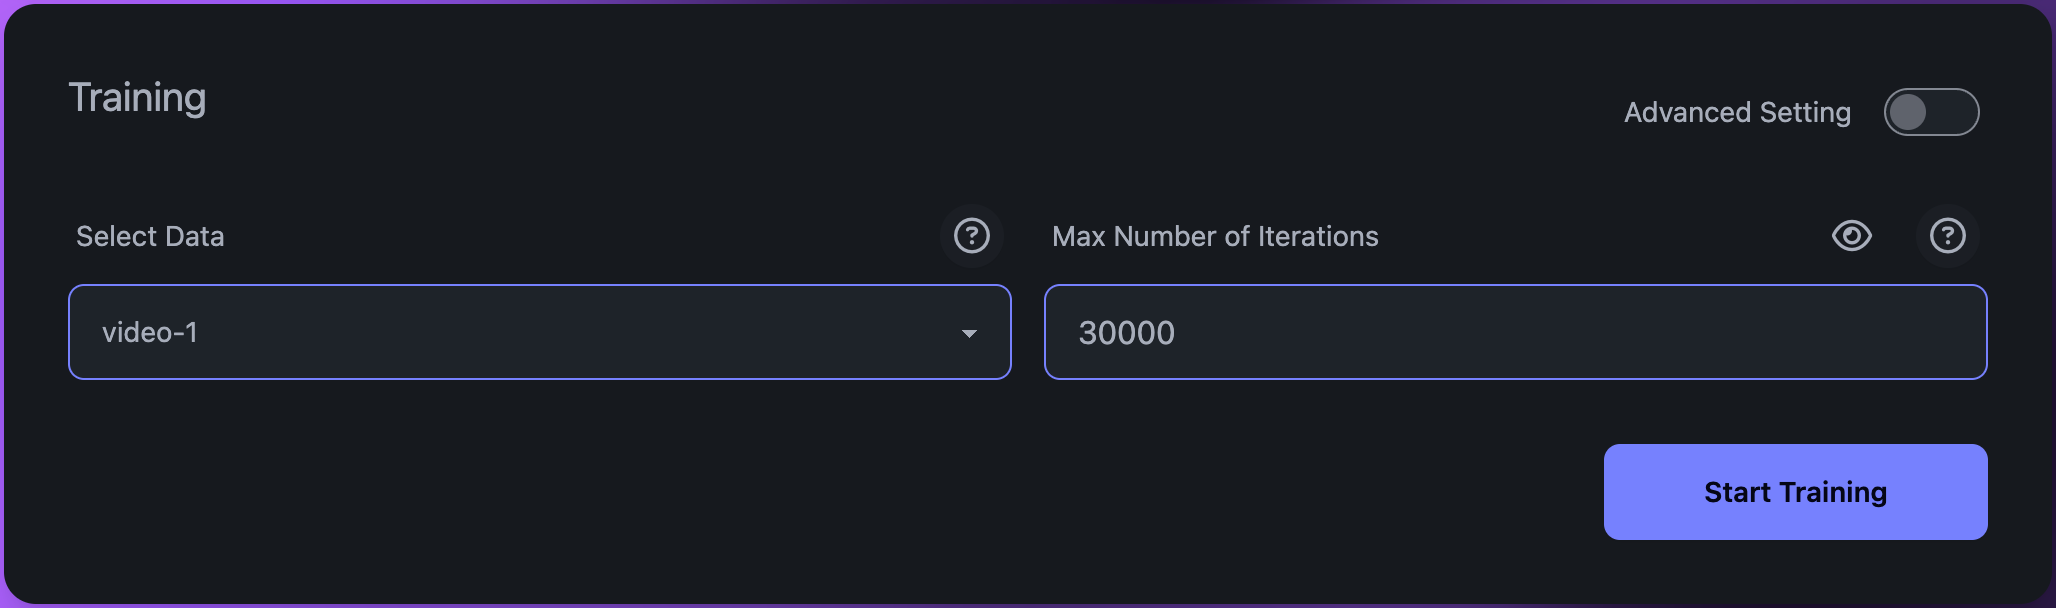
\includegraphics[width=\textwidth]{figures/fix-2.png}
	\caption{Consistent Wording for Training Button}
  \label{fig:fix-2}
\end{figure}

\paragraph{Enhanced Project Creation}
The project creation process was moved into a modal dialog, which not only eliminates a point of confusion but also clarified the need to name projects before creation \fref{fig:fix-3}.

\begin{figure}[htb]
	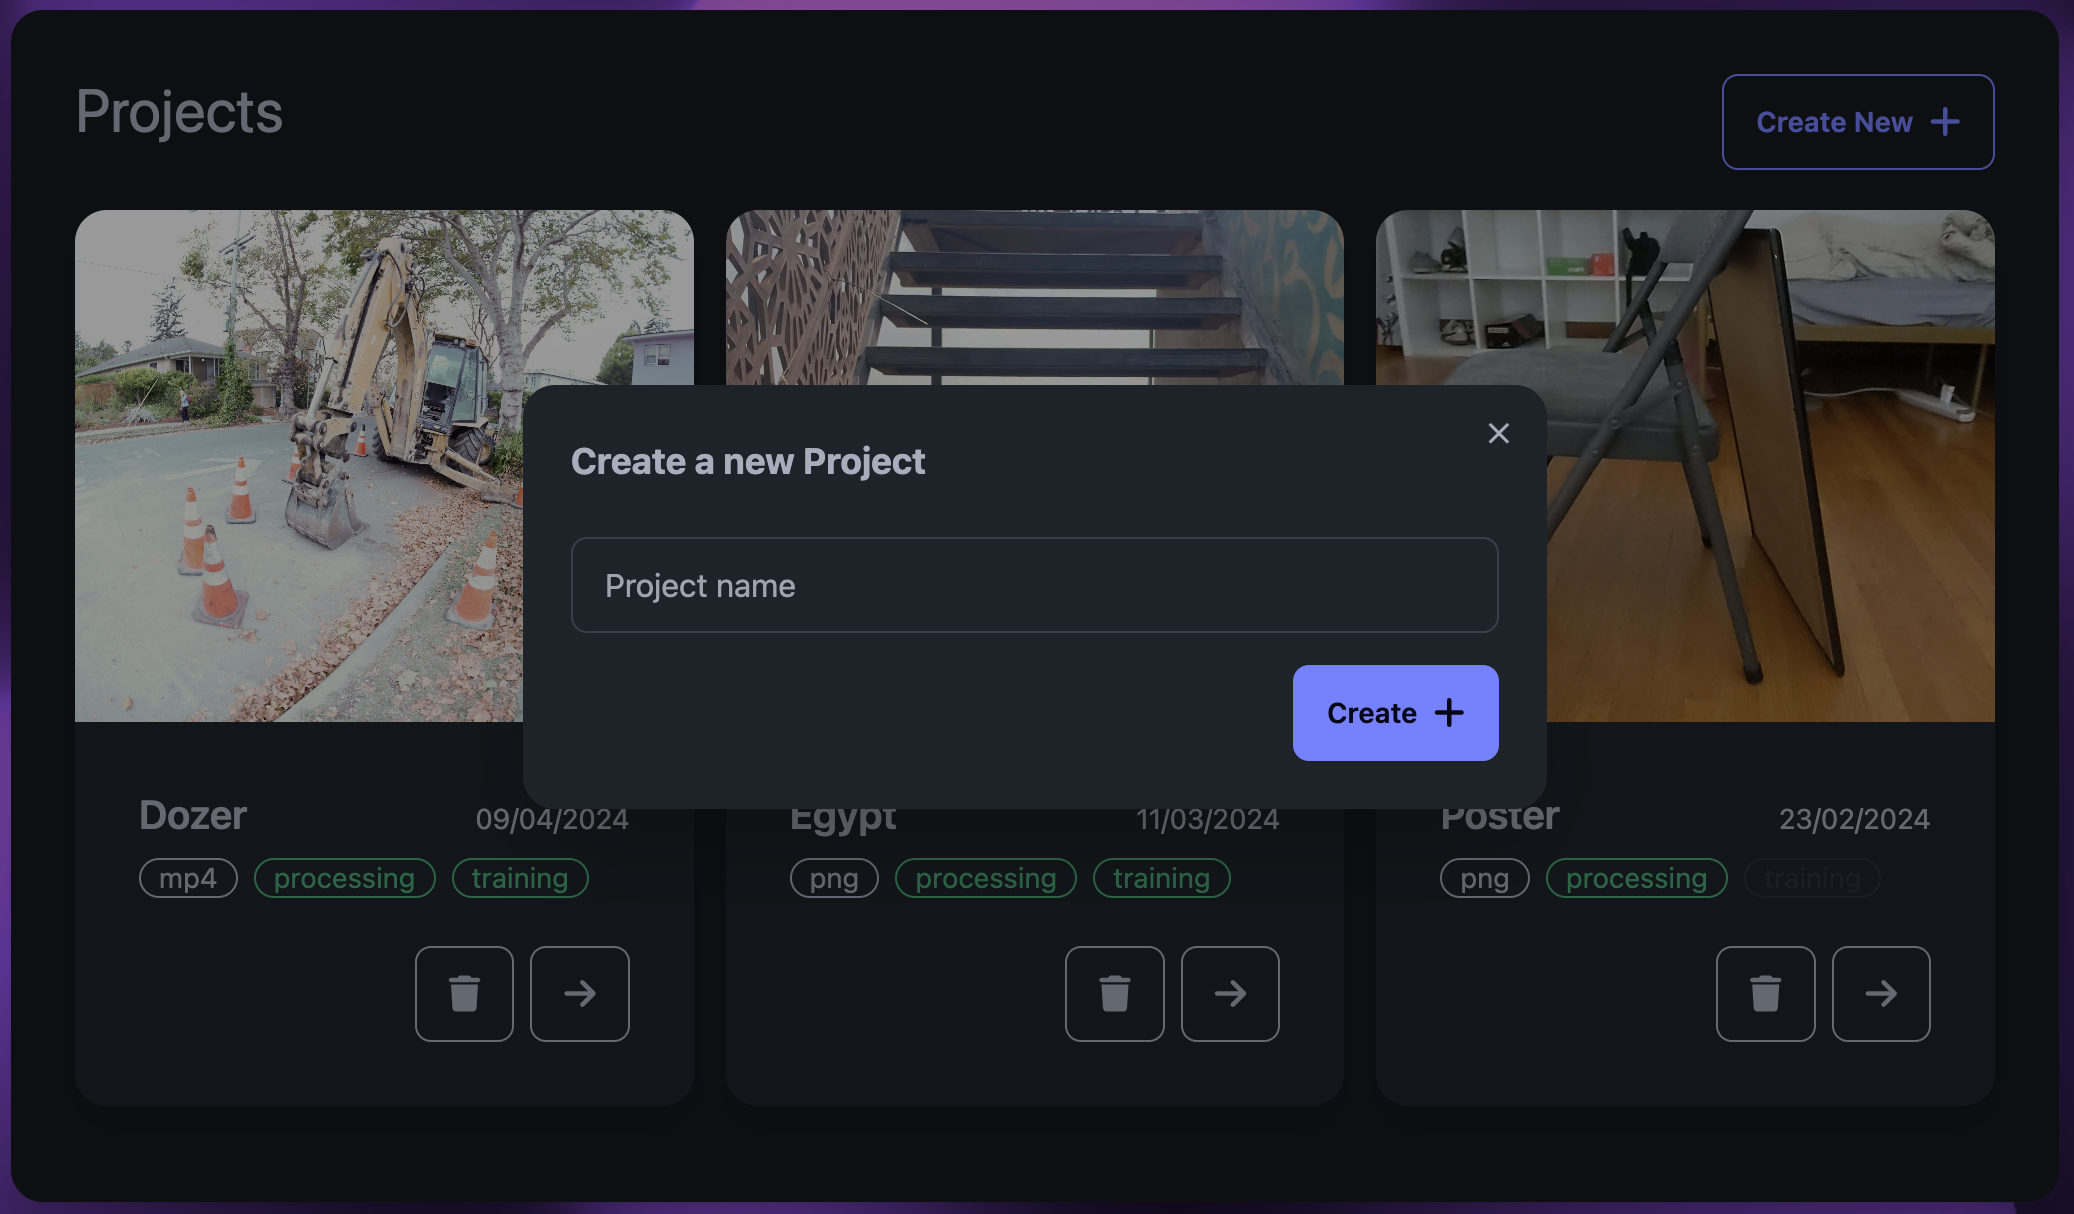
\includegraphics[width=\textwidth]{figures/fix-3.png}
	\caption{Modal Dialog for Project Creation}
  \label{fig:fix-3}
\end{figure}

\paragraph{File Upload Improvements}
The file upload process was improved by adding some guardrails, to ensure user would not accidentally skip a step. 
The upload button starts out disabled, so that the only interactive element is the file-input field.
Once a file is selected, the button becomes active, indicating to the user that they can proceed to upload their selected file.
Only one the file is uploaded, the UI elements related to pre-processing appear, guiding the user through the next steps. 
This solution is likely to prevent many of the issues users encountered when uploading files during testing. \fref{fig:fix-4}


\begin{figure}[htb]
  \begin{subfigure}{\textwidth}
    \centering
    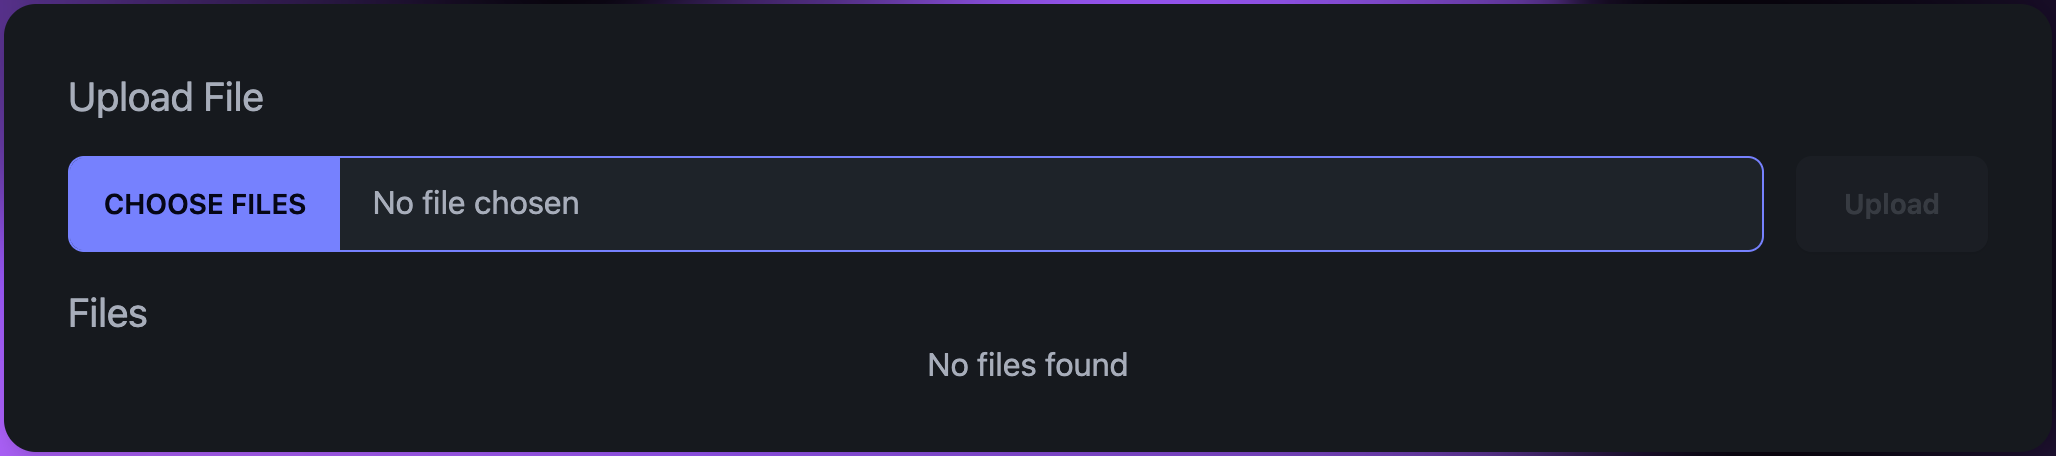
\includegraphics[width=.8\linewidth]{figures/fix-4.1.png}
    \caption{Initial State}
  \end{subfigure}
  \begin{subfigure}{\textwidth}
    \centering
    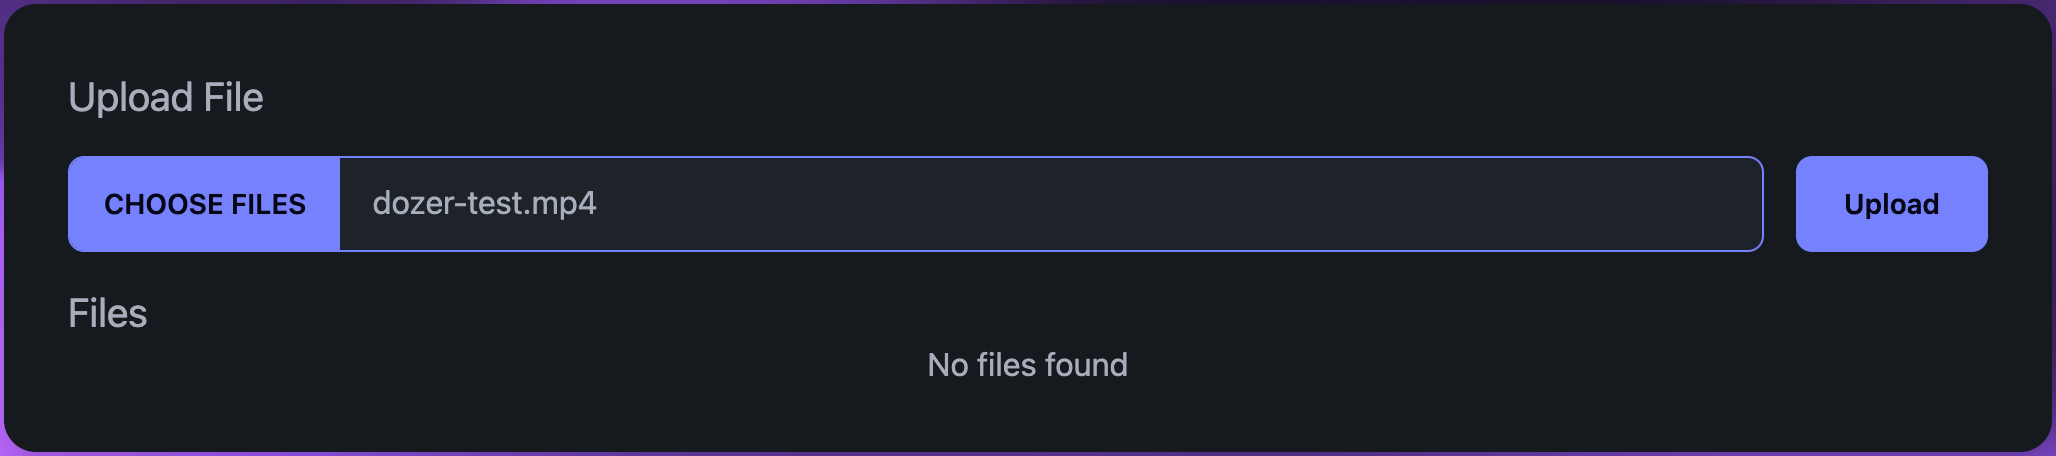
\includegraphics[width=.8\linewidth]{figures/fix-4.2.png}
    \caption{File Selected}
  \end{subfigure}
  \begin{subfigure}{\textwidth}
    \centering
    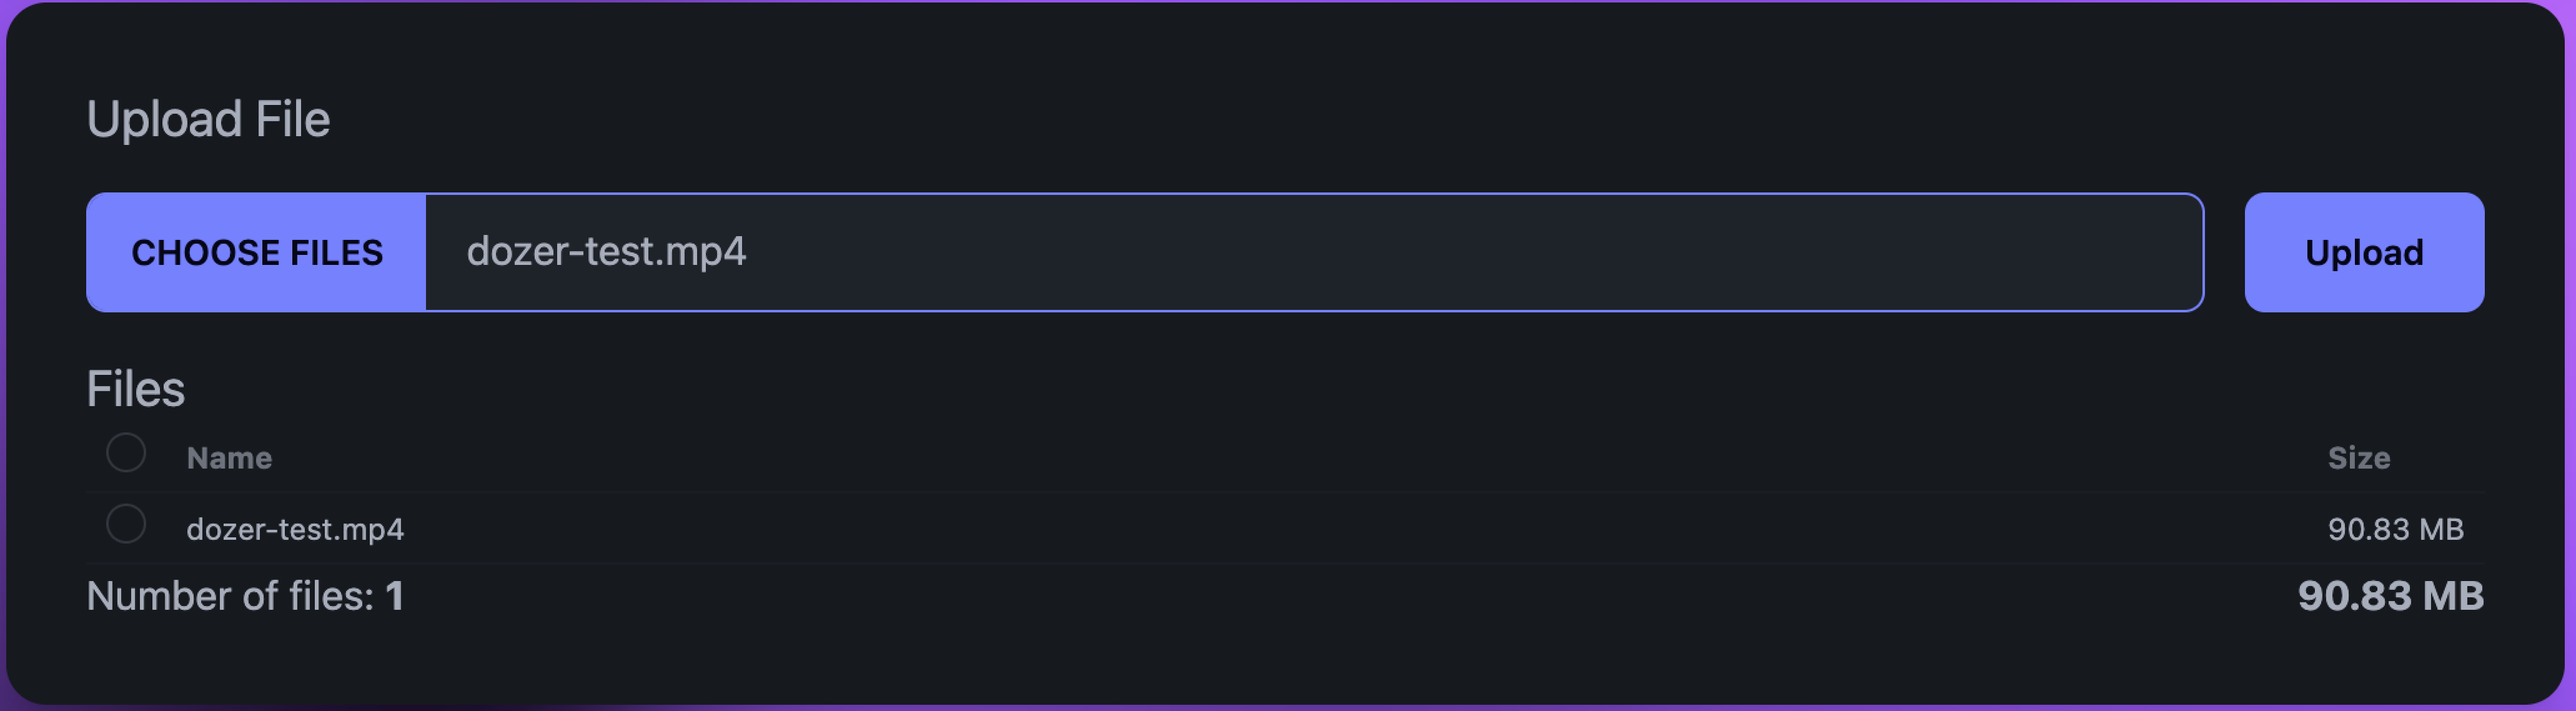
\includegraphics[width=.8\linewidth]{figures/fix-4.3.png}
    \caption{File Uploaded}
  \end{subfigure}
	\caption{Improved File Upload Process}
  \label{fig:fix-4}
\end{figure}
